\section{实验参数设置}
本文设定的实验场景为$1.2\times 1.2~m$封闭环境,除四周墙壁外不设置任何其他障碍。在程序启动时同时载入学习鼠和规则鼠,其中学习鼠用黄色标识,规则鼠用红色标识,这一颜色只用于场景展示,对机器鼠行为决策无意义。学习鼠与规则鼠的初始中心距离$d_{cc}$为$1.0~m$,位置分别为$[0,0]$(规则鼠)和$[0,1]$(学习鼠),头部均朝向$x$正方向(图\ref{figure_expsetup})。
%\begin{enumerate}[leftmargin=0em, listparindent=2em, parsep=0em, topsep=0em, label=(\theenumi)]
%%\setlength{\leftmargin}{0em}
%\setlength{\itemindent}{4em}
%\setlength{\labelsep}{0em}
%\setlength{\labelwidth}{2em}
%\setlength{\parsep}{0em}
%\setlength{\itemsep}{0em}
%\setlength{\topsep}{0em}
%%\setlength{\listparindent}{2em}
%  \item 学习鼠,位置:$[0,0]$
%  \item 利用ROS搭建了用于行为交互的仿真平台,该平台各层相互解耦,具有良好的可扩展性和较强的鲁棒性。
%  \item 在机器鼠行为交互中应用Q-学习算法,部分解决了传统
%\end{enumerate}
\begin{figure}[htb]
  %\vspace{13pt}
  \centering
  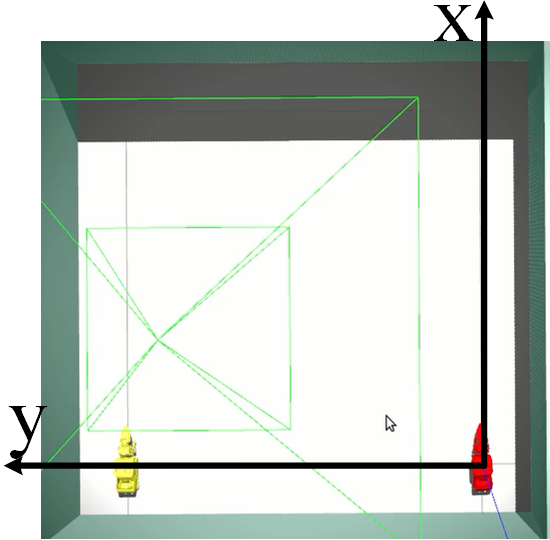
\includegraphics[width=7cm]{images/ch05/expsetup.png}
  \caption{实验启动界面}\label{figure_expsetup}
\end{figure}

本文只考虑仿生机器鼠在行为交互活动种的表现,不考虑模拟生物鼠表现的进食、饮水、睡眠等行为,因此实验场景中不设置食物和水源等。

训练开始时,学习鼠的Q表以0填充,这表示其不具备任何先验知识,全部状态-动作组均需进行探索和更新。当实验开始后,系统会随时存储Q表,以便实验中止后能够从断点继续训练。

其他与学习鼠行为决策相关的参数和设定分别为:
\begin{enumerate}[leftmargin=0em, listparindent=2em, parsep=0em, topsep=0em, label=(\theenumi)]
%\setlength{\leftmargin}{0em}
\setlength{\itemindent}{4em}
\setlength{\labelsep}{0em}
\setlength{\labelwidth}{2em}
\setlength{\parsep}{0em}
\setlength{\itemsep}{0em}
\setlength{\topsep}{0em}
%\setlength{\listparindent}{2em}
  \item 贪心率$\epsilon=0.2$。
  \item 学习率$\alpha=0.8$。
  \item 遗忘率$\gamma=0.8$。
  \item 终止状态$terminal-state$:$s_5$梳理或$s_6$被梳理。%系统到达最终状态后会发布自上一次最终状态以来累积的即时奖励和。
\end{enumerate}

